\section{Restrictions}
\label{sec:restrictions}

It was found in the interviews in \cref{sub:administersinterviews} and with our industry partner in \cref{sec:fabrikken}, that the venues have a strong desire for the ability control, what guests can vote for. This was valued to be a must have and of high priority. A possible concept for solving the this problem, is by putting restrictions on what tracks, can be added to the playlist. This section will present the the concepts of white- and black-listing.

\paragraph{Whitelisting} is a concept of being able to choose, what entities is a accepted as a valid input. Strictly if $A$ is the set of accepted inputs, $B$ is the whitelist set and $i$ is the input then $i \in A$ \textbf{if and only if} $i \in B$. There can be multiple whitelist if input is in either of them, it is valid, \cref{fig:restrictions}.

\paragraph{Blacklisting} is the reverse of whitelisting. The concept is that the blacklist excludes specific entities from being a valid input. Entities in the blacklist set is excluded from the set of accepted inputs. Strictly $A$ is the set of accepted inputs, $B$ is the blacklist set and $i$ is the input set then $i \in A$ \textbf{if and only if} $i \notin B$.


\begin{figure}[H]
  \centering
  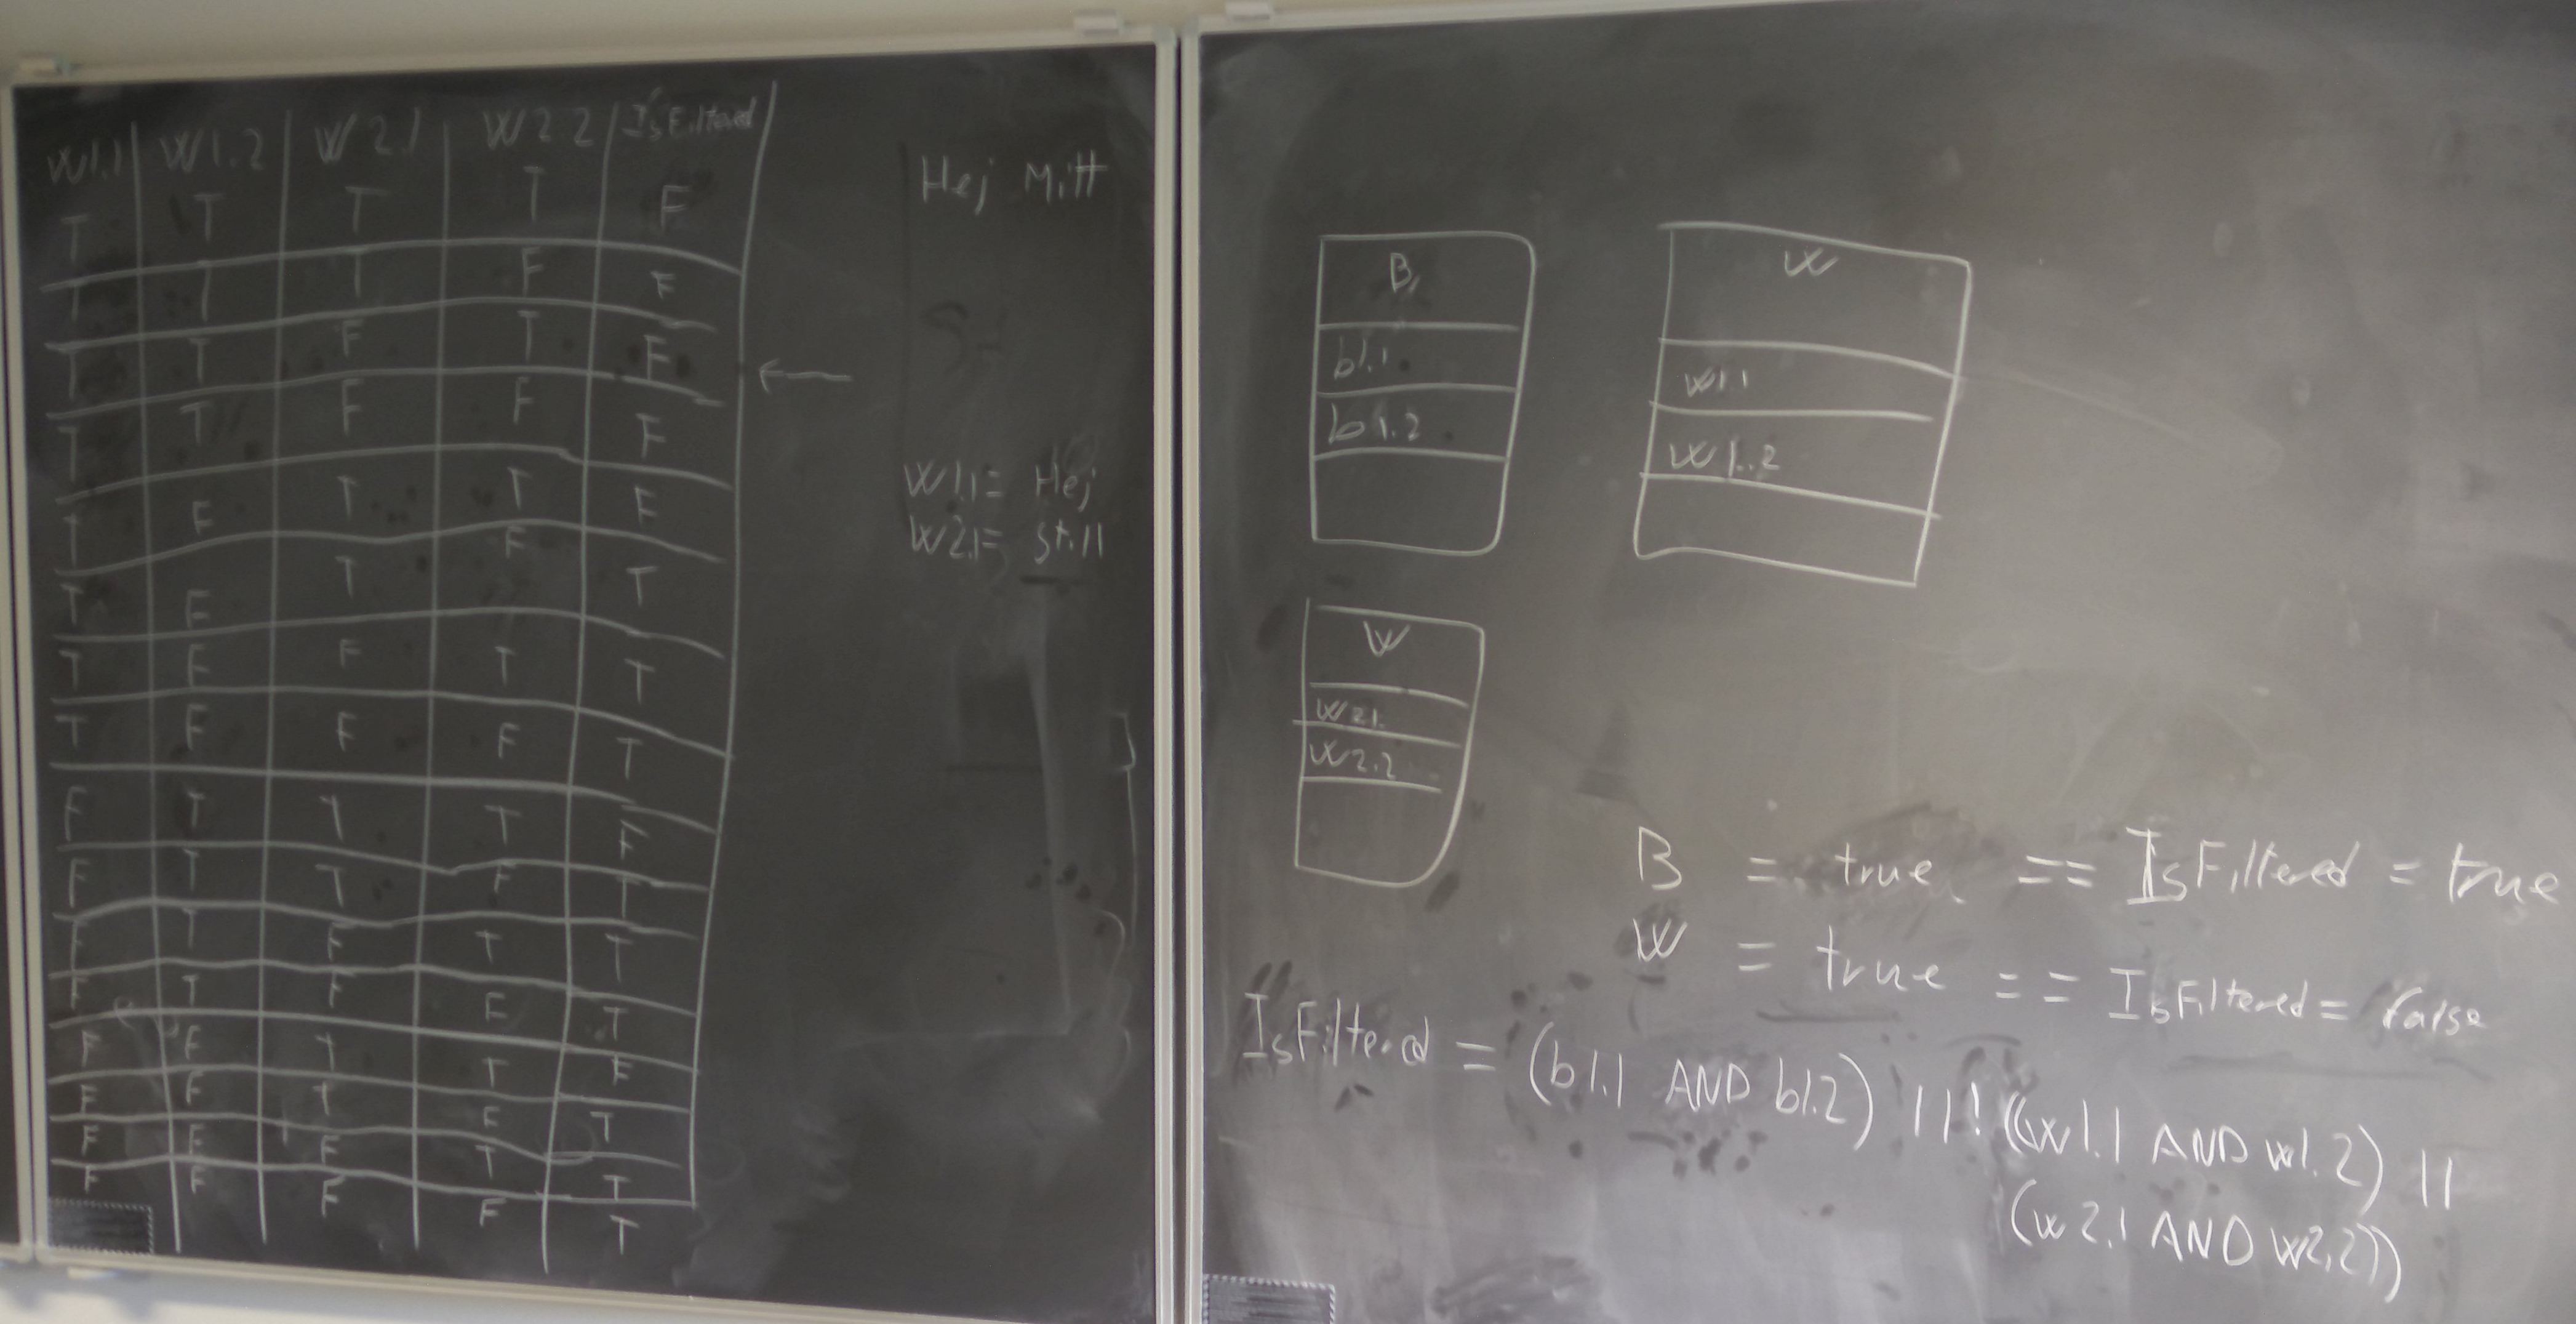
\includegraphics[width=1.2\linewidth]{Images/restriction.jpg}
  \caption{Truthtable of multiple whitelists.}\label{fig:restrictions}
\end{figure}

With these concepts it is possible to restrict the music catalogue to a subset of allowed tracks, satifying the requirement of being able to control what music is being played. Restrictions can also improve the music flow (described in \cref{sub:MusicFlow}) if the restrictions limits allowed tracks to certain genre or mood, although this should be just be supplement to another concept, analysing the tracks on the playlist.

Futher more the owner of Fabrikken\cref{sec:fabrikken} wanting to be able to have timed intervals of restrictions, so that the restrictions acts accordingly to the progression in intensity and mood of the bar environment. This is quite trivially implemented with a selective control structure, checking if the restriction is relevant at that time of day.